% !TeX document-id = {31cec06c-209e-42c6-b48d-393b1a0af1d2}
% !TeX TS-program = xelatex
% !BIB TS-program = biber
% !TeX encoding = UTF-8
% !TeX spellcheck = en_US
% !TeX root = seminar_presentation__intelligent_industrial_robots.tex


%% LaTeX-Beamer template for KIT design
%% by Erik Burger, Christian Hammer
%% title picture by Klaus Krogmann
%%
%% version 2.1
%%
%% mostly compatible to KIT corporate design v2.0
%% http://intranet.kit.edu/gestaltungsrichtlinien.php
%%
%% Problems, bugs and comments to
%% burger@kit.edu

\documentclass[18pt]{beamer}

\usepackage[utf8]{inputenc}

%% SLIDE FORMAT

% use 'beamerthemekit' for standard 4:3 ratio
% for widescreen slides (16:9), use 'beamerthemekitwide'
% for widescreen slide without sidebar use 'beamerthemekitwidenosidebar'

%\usepackage{templates/beamerthemekit}
%\usepackage{templates/beamerthemekitwide}
\usepackage{templates/beamerthemekitwidenosidebar}

% use this to disable the latex beamer navigation symbols
%\beamertemplatenavigationsymbolsempty


%% TITLE PICTURE

% if a custom picture is to be used on the title page, copy it into the 'logos'
% directory, in the line below, replace 'mypicture' with the 
% filename (without extension) and uncomment the following line
% (picture proportions: 63 : 20 for standard, 169 : 40 for wide
% *.eps format if you use latex+dvips+ps2pdf, 
% *.jpg/*.png/*.pdf if you use pdflatex)

\titleimage{plc_logo}

%% TITLE LOGO

% for a custom logo on the front page, copy your file into the 'logos'
% directory, insert the filename in the line below and uncomment it

\titlelogo{iar_iirob}

% (*.eps format if you use latex+dvips+ps2pdf,
% *.jpg/*.png/*.pdf if you use pdflatex)

%% TikZ INTEGRATION

% use these packages for PCM symbols and UML classes
\usepackage{templates/tikzkit}
\usepackage{templates/tikzuml}

\usepackage{tabularx}
\usepackage{multirow}
\usepackage{multicol}
\usepackage{booktabs}

% the presentation starts here

\title[Automated Programming of Programmable Logic Controllers]{Seminar Intelligent Industrial Robots}
\subtitle{Automated Programming of Programmable Logic Controllers}
\author{David Oberacker}

\institute{
	Institute for Anthropomatics and Robotics - Intelligent Process Automation and Robotics Lab (IAR-IPR)
}

% Bibliography

\usepackage[citestyle=authoryear,bibstyle=numeric,hyperref,backend=biber]{biblatex}
\addbibresource{presentation.bib}
\bibhang1em

\begin{document}

% change the following line to "ngerman" for German style date and logos
\selectlanguage{english}

%title page
\begin{frame}
\titlepage
\end{frame}

%table of contents
\begin{frame}{Outline}
\tableofcontents
\end{frame}

\section{Introduction}

%\begin{frame}{Introduction}
%    \begin{figure}
%        \centering
%        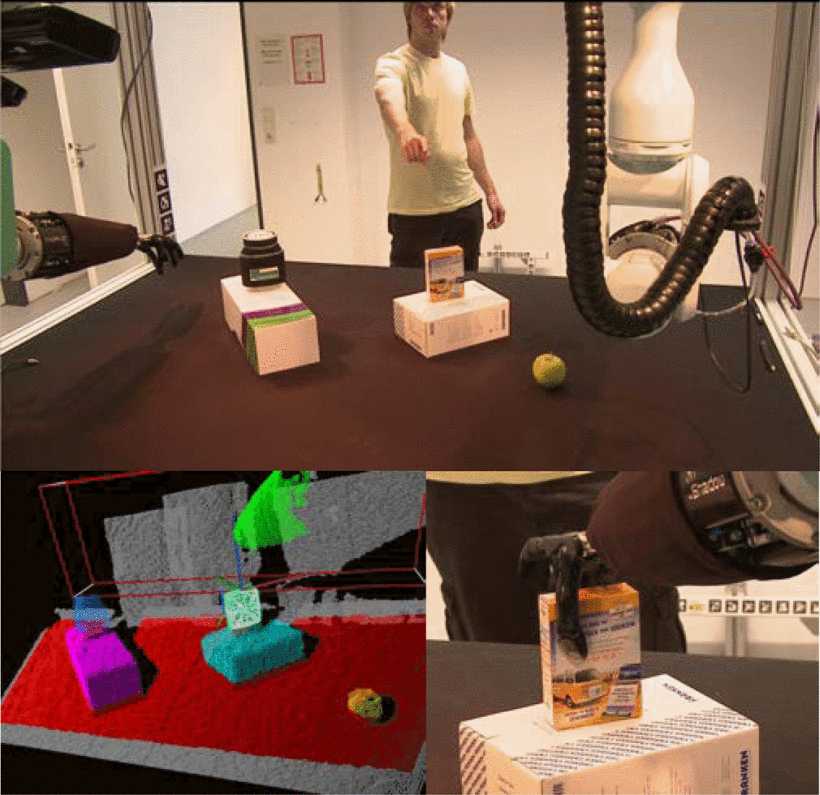
\includegraphics[height=0.7\textheight]{figures/3d_semantic_grasping.png}
%    \end{figure}
%\footcitetext{6385692}
%\end{frame}

\begin{frame}{Introduction}
    

    \begin{itemize}
        \item Grasping of moving object is one of important operations for modern robots.
        \item Objects have to be \textbf{detected} and \textbf{localized}.
        \item Semantic segmentation can be used $\rightarrow$ Multiple instances of same class can not be distinguished.
    \end{itemize}
    $\Rightarrow $ Are state of the art instance segmentation algorithms viable for real-time applications ?
    
\end{frame}

\section{Programmable logic controller}

\begin{frame}{Programmable Logic Controller}
\begin{columns}
    \begin{column}{0.5\textwidth}
        \begin{itemize}
            \item Every Pixel is labeled.
            \item Instances of the same class \textbf{can not be distinguished}.
            \item Decoder-encoder architecture.
            \item Commonly used architectures:
            \begin{itemize}
                \item DeepLabV3~\footnotemark
                
                \item SegNet~\footnotemark
                
            \end{itemize}
        \end{itemize}
    \end{column}
    \begin{column}{0.5\textwidth}
        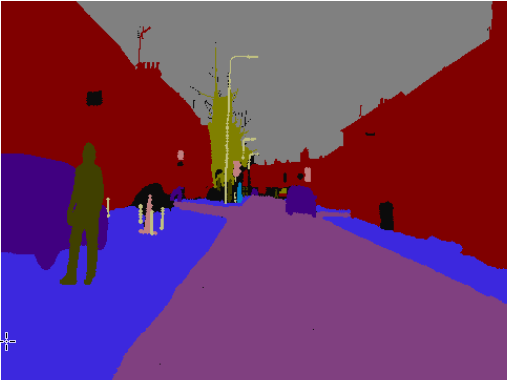
\includegraphics[width=\textwidth]{figures/segnet_example.png}
    \end{column}
\end{columns}
\footcitetext{DBLP:journals/corr/abs-1802-02611}
\footcitetext{DBLP:journals/corr/BadrinarayananK15}
\end{frame}

\subsection{IEC 61131-3 Languages}

\begin{frame}{Ladder Diagram}
\begin{columns}
	\begin{column}{0.5\textwidth}
		\begin{itemize}
			\item Every Pixel is labeled.
			\item Different instances of the same class \textbf{are separated}.
			\item More complex pipelines.
			\item Commonly used architectures:
			\begin{itemize}
				\item Mask R-CNN~\footnotemark
				\item Hybrid Task Cascade~\footnotemark
				\item ESE-Seg~\footnotemark
			\end{itemize}
		\end{itemize}
	\end{column}
	\begin{column}{0.5\textwidth}
		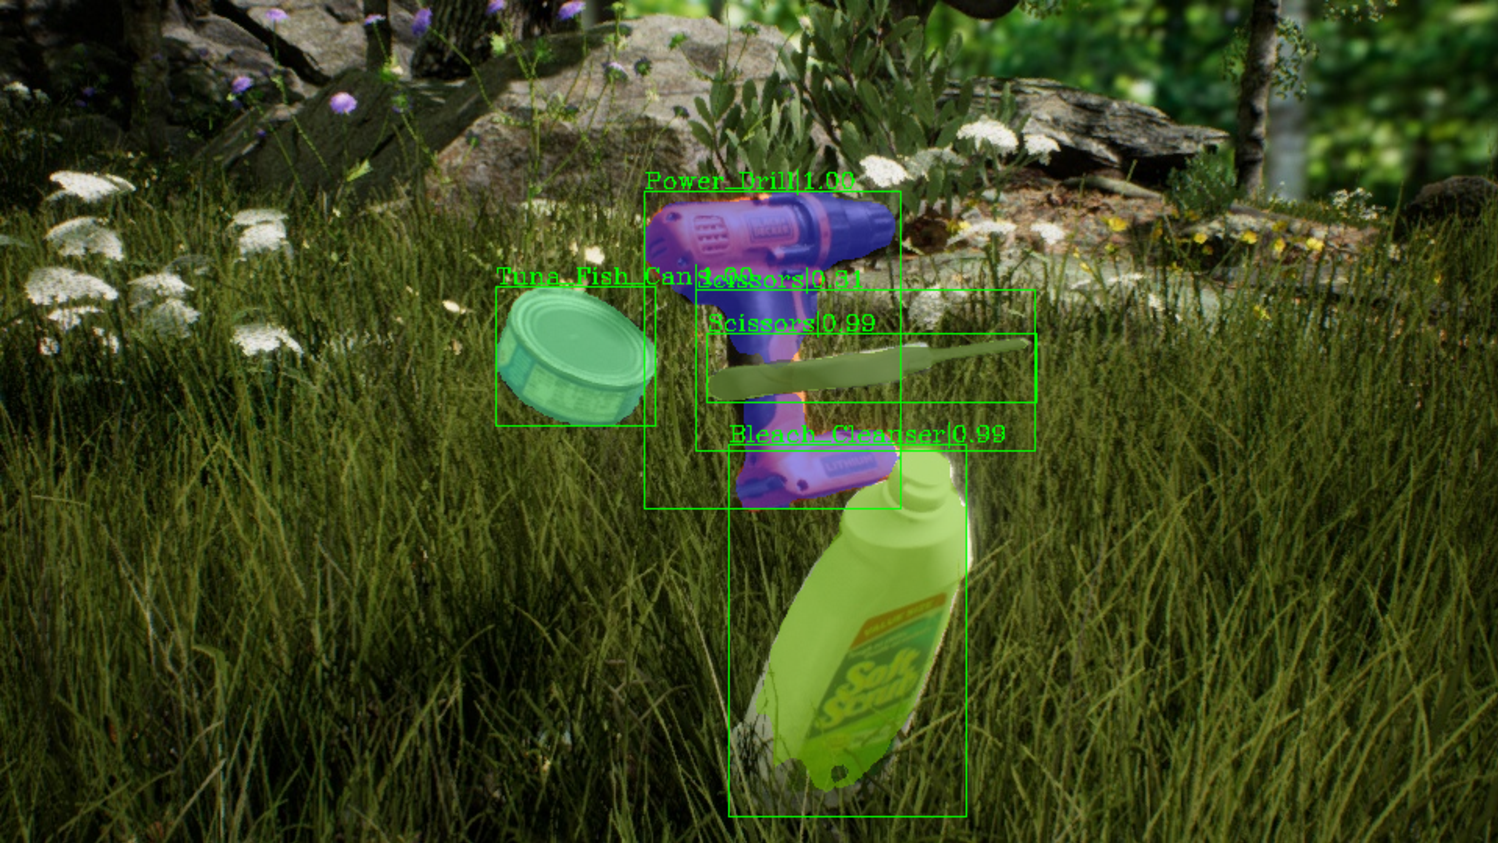
\includegraphics[width=\textwidth]{figures/cmrcnn_mobilenet_fat.pdf}
	\end{column}
\end{columns}
\footcitetext{DBLP:journals/corr/HeGDG17}
\footcitetext{DBLP:journals/corr/abs-1901-07518}
\footcitetext{2019arXiv190804067X}
\end{frame}

\begin{frame}{Structured Text}
    \begin{columns}
        \begin{column}{0.5\textwidth}
           \begin{itemize}
               \item Every Pixel is labeled.
               \item Different instances of the same class \textbf{are separated}.
               \item More complex pipelines.
               \item Commonly used architectures:
               \begin{itemize}
                   \item Mask R-CNN~\footnotemark
                   \item Hybrid Task Cascade~\footnotemark
                   \item ESE-Seg~\footnotemark
               \end{itemize}
           \end{itemize}
        \end{column}
        \begin{column}{0.5\textwidth}
            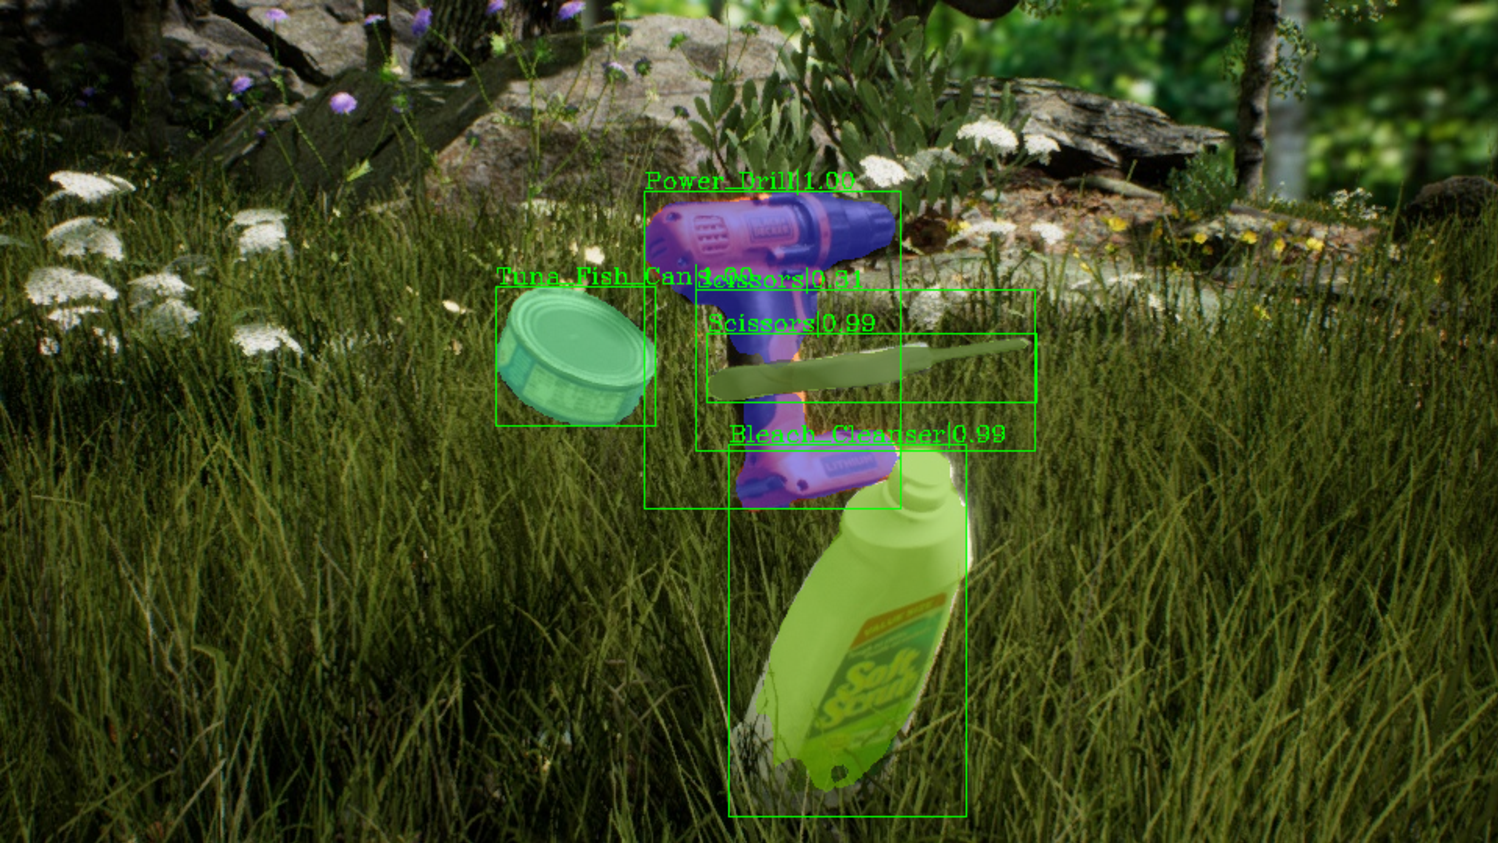
\includegraphics[width=\textwidth]{figures/cmrcnn_mobilenet_fat.pdf}
        \end{column}
\end{columns}
\footcitetext{DBLP:journals/corr/HeGDG17}
\footcitetext{DBLP:journals/corr/abs-1901-07518}
\footcitetext{2019arXiv190804067X}
\end{frame}

\section{Automated programming of PLCs}

\begin{frame}{Datasets}
\begin{itemize}
    \item Common Objects in Context (COCO)
    \begin{itemize}
        \item 115 000 annotated images.
        \item Indoor and outdoor scenes.
        \item 80 foreground object classes.
    \end{itemize}
    \item Falling Things Dataset (FAT)
    \begin{itemize}
        \item 60 000 annotated images.
        \item Synthetic dataset.
        \item Objects failing through synthetic backgrounds.
    \end{itemize}
    \item YCB Video Dataset (YCB)
    \begin{itemize}
        \item 12 000 annotated images.
        \item Video frames from a camera pan around objects.
        \item Same objects as in the FAT dataset.
    \end{itemize}
\end{itemize}
\end{frame}

\subsection{C/C++-based programming}

\begin{frame}{Datasets}
\begin{itemize}
	\item Common Objects in Context (COCO)
	\begin{itemize}
		\item 115 000 annotated images.
		\item Indoor and outdoor scenes.
		\item 80 foreground object classes.
	\end{itemize}
	\item Falling Things Dataset (FAT)
	\begin{itemize}
		\item 60 000 annotated images.
		\item Synthetic dataset.
		\item Objects failing through synthetic backgrounds.
	\end{itemize}
	\item YCB Video Dataset (YCB)
	\begin{itemize}
		\item 12 000 annotated images.
		\item Video frames from a camera pan around objects.
		\item Same objects as in the FAT dataset.
	\end{itemize}
\end{itemize}
\end{frame}

\subsection{Formal description based}

\begin{frame}{Linear Temporal Logic}
\begin{itemize}
	\item Common Objects in Context (COCO)
	\begin{itemize}
		\item 115 000 annotated images.
		\item Indoor and outdoor scenes.
		\item 80 foreground object classes.
	\end{itemize}
	\item Falling Things Dataset (FAT)
	\begin{itemize}
		\item 60 000 annotated images.
		\item Synthetic dataset.
		\item Objects failing through synthetic backgrounds.
	\end{itemize}
	\item YCB Video Dataset (YCB)
	\begin{itemize}
		\item 12 000 annotated images.
		\item Video frames from a camera pan around objects.
		\item Same objects as in the FAT dataset.
	\end{itemize}
\end{itemize}
\end{frame}

\begin{frame}{UML / SysML}
\begin{itemize}
	\item Common Objects in Context (COCO)
	\begin{itemize}
		\item 115 000 annotated images.
		\item Indoor and outdoor scenes.
		\item 80 foreground object classes.
	\end{itemize}
	\item Falling Things Dataset (FAT)
	\begin{itemize}
		\item 60 000 annotated images.
		\item Synthetic dataset.
		\item Objects failing through synthetic backgrounds.
	\end{itemize}
	\item YCB Video Dataset (YCB)
	\begin{itemize}
		\item 12 000 annotated images.
		\item Video frames from a camera pan around objects.
		\item Same objects as in the FAT dataset.
	\end{itemize}
\end{itemize}
\end{frame}

\begin{frame}{Simulink}
\begin{itemize}
	\item Common Objects in Context (COCO)
	\begin{itemize}
		\item 115 000 annotated images.
		\item Indoor and outdoor scenes.
		\item 80 foreground object classes.
	\end{itemize}
	\item Falling Things Dataset (FAT)
	\begin{itemize}
		\item 60 000 annotated images.
		\item Synthetic dataset.
		\item Objects failing through synthetic backgrounds.
	\end{itemize}
	\item YCB Video Dataset (YCB)
	\begin{itemize}
		\item 12 000 annotated images.
		\item Video frames from a camera pan around objects.
		\item Same objects as in the FAT dataset.
	\end{itemize}
\end{itemize}
\end{frame}

\begin{frame}{plcSpecif}
\begin{itemize}
	\item Common Objects in Context (COCO)
	\begin{itemize}
		\item 115 000 annotated images.
		\item Indoor and outdoor scenes.
		\item 80 foreground object classes.
	\end{itemize}
	\item Falling Things Dataset (FAT)
	\begin{itemize}
		\item 60 000 annotated images.
		\item Synthetic dataset.
		\item Objects failing through synthetic backgrounds.
	\end{itemize}
	\item YCB Video Dataset (YCB)
	\begin{itemize}
		\item 12 000 annotated images.
		\item Video frames from a camera pan around objects.
		\item Same objects as in the FAT dataset.
	\end{itemize}
\end{itemize}
\end{frame}

\begin{frame}{GRAFCET}
\begin{itemize}
	\item Common Objects in Context (COCO)
	\begin{itemize}
		\item 115 000 annotated images.
		\item Indoor and outdoor scenes.
		\item 80 foreground object classes.
	\end{itemize}
	\item Falling Things Dataset (FAT)
	\begin{itemize}
		\item 60 000 annotated images.
		\item Synthetic dataset.
		\item Objects failing through synthetic backgrounds.
	\end{itemize}
	\item YCB Video Dataset (YCB)
	\begin{itemize}
		\item 12 000 annotated images.
		\item Video frames from a camera pan around objects.
		\item Same objects as in the FAT dataset.
	\end{itemize}
\end{itemize}
\end{frame}

\section{Risks of automated programming}

\begin{frame}{Transformation function correctness}

\begin{block}{Transformation function correctness}
	\begin{itemize}
		\item Processing time is strongly bound to the architecture.
		\item Optimizing the processing times is a important topic for modern architectures.
	\end{itemize}
\end{block}
\end{frame}

\begin{frame}{Runtime guarantees}

\begin{block}{Runtime guarantees}
	\begin{itemize}
		\item Processing time is strongly bound to the architecture.
		\item Optimizing the processing times is a important topic for modern architectures.
	\end{itemize}
\end{block}
\end{frame}

\section{Conclusions}
\begin{frame}{Conclusions}

\begin{block}{Processing Time Profiling}
	\begin{itemize}
		\item Processing time is strongly bound to the architecture.
		\item Optimizing the processing times is a important topic for modern architectures.
	\end{itemize}
\end{block}
\pause
\begin{block}{Household Object Robot Grasping}
    \begin{itemize}
        \item Qualitative results are promising for future research.
        \item Robustness has to be improved for real world aplications.
        \item Dataset selection is relevant for result quality.
        \item When looking at functional safety, the current evaluation methods are not sufficient.
    \end{itemize}
\end{block}
\end{frame}

\begin{frame}
\vfill
\centering
{\LARGE Thank you for your attention.}\\
\vspace{1cm}
{\Large \textbf{Questions ?}}
\vfill
\end{frame}

\appendix
\beginbackup

\nocite{*}

\begin{frame}[allowframebreaks]{References}
\printbibliography
\end{frame}

\backupend

\end{document}
\grid
